\subsection{Moving frame for \KSe}

The first few fundamental invariants for the action\ES{This action will be written in KSe symmetries chapter, then I will just refer to it here} of $\SOn{2}\subset\On{2}$ on the phase space
of \KSe\ have been tabulated in \reftab{tab:SO2n6}. The obvious singularity at $b_1=c_1=0$ can be
corrected by substituting $r_1$ with $r=\sum_{i=1}^3 b_i^2+c_i^2$ in the denominators. The reason
for using only the first three mode magnitudes is that this choice is enough to prevent the denominator from vanishing at one of the three equilibria $E_i$, $i=1\ldots3$. With this modification one has to note that the invariants of \reftab{tab:SO2n6} vanish at \EQB{2} and \EQB{3}. In principle this is not a problem since we want to carry out reduction in the principal stratum. In practice this causes two important equilibria to be mapped to the origin and leads to \statesp\ portraits as in \reffig{fig:ksSO2eqbTo0}. The neighborhood of \EQB{2} and \EQB{3} which is where we would like to get some intuition about the behavior of \rpo s, has been squeezed into a cone-shaped surface.

%%%%%%%%%%%%%%%%%%%%%%%%%%%%%%%%%%%%%%%%%%%%%%%%%%%%%%%%%%%%%%%%%%
\begin{figure}[t]
\begin{center}
  (\textit{a})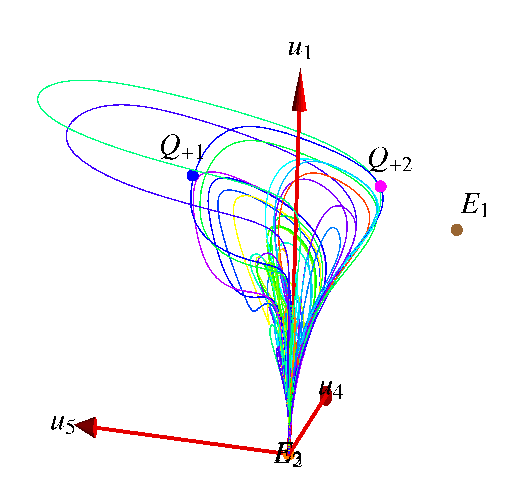
\includegraphics[width=0.4\textwidth]{../figs/ksSO2inv145eqbTo0.eps}
\end{center}
\caption[KSe SO(2) reduced phase space with modified invariants.]{ Phase space portrait of $L=22$ \KS\ dynamics projected to invariants given in \reftab{tab:SO2n6}. The trajectories shown are 20 short \rpo s.
   }
\label{fig:ksSO2eqbTo0}
\end{figure}
%%%%%%%%%%%%%%%%%%%%%%%%%%%%%%%%%%%%%%%%%%%%%%%%%%%%%%%%%%%%%%%%

To overcome this problem we modify the invariants of  \reftab{tab:SO2n6} as follows. We observe that the invariants come as either symmetric or antisymmetric under the action of $\Dn{1}\subset\On{2}$. We modify the symmetric invariants by adding a term $\sqrt{b_i^2+c_i^2}$ where $i$ the corresponding irreducible subspace  (Fourier mode). The new invariants are listed in \reftab{tab:SO2n6modif}.

\begin{table}
\begin{small}
\begin{eqnarray*}
  u_1=r_1 &=&\sqrt{b_1^2+c_1^2}\\ 
  u_3 &=&\frac{b_2 \left(b_1^2-c_1^2\right)+2 b_1 c_1 c_2}{r^2}\\ 
  u_4 &=&\sqrt{b_2^2+c_2^2}+\frac{-2
b_1 b_2 c_1+\left(b_1^2-c_1^2\right) c_2}{r^2}\\ 
  u_5 &=&\sqrt{b_3^2+c_3^2}+\frac{b_1 b_3 \left(b_1^2-3 c_1^2\right)-c_1 \left(-3
b_1^2+c_1^2\right) c_3}{r^3}\\ 
  u_6 &=&\frac{-3 b_1^2 b_3 c_1+b_3 c_1^3+b_1^3 c_3-3 b_1 c_1^2 c_3}{r^3}\\
  u_7 &=&\frac{b_4
\left(b_1^4-6 b_1^2 c_1^2+c_1^4\right)+4 b_1 c_1 \left(b_1^2-c_1^2\right) c_4}{r^4}\\
  u_8 &=&\sqrt{b_4^2+c_4^2}+\frac{4 b_1
b_4 c_1 \left(-b_1^2+c_1^2\right)+\left(b_1^4-6 b_1^2 c_1^2+c_1^4\right) c_4}{r^4}\\ 
  u_9 &=&\sqrt{b_5^2+c_5^2}+\frac{b_1
b_5 \left(b_1^4-10 b_1^2 c_1^2+5 c_1^4\right)+c_1 \left(5 b_1^4-10 b_1^2 c_1^2+c_1^4\right) c_5}{r^5}\\ 
  u_{10} &=&\frac{-b_5
c_1 \left(5 b_1^4-10 b_1^2 c_1^2+c_1^4\right)+b_1 \left(b_1^4-10 b_1^2 c_1^2+5 c_1^4\right) c_5}{r^5}\\  
  u_{11} &=&\frac{b_6
\left(b_1^6-15 b_1^4 c_1^2+15 b_1^2 c_1^4-c_1^6\right)+2 b_1 c_1 \left(3 b_1^4-10 b_1^2 c_1^2+3 c_1^4\right) c_6}{r^6} \\
  u_{12} &=&\sqrt{b_6^2+c_6^2}+\frac{-2
b_1 b_6 c_1 \left(3 b_1^4-10 b_1^2 c_1^2+3 c_1^4\right)+\left(b_1^6-15 b_1^4 c_1^2+15 b_1^2 c_1^4-c_1^6\right) c_6}{r^6} 
\end{eqnarray*}
\caption[Modified invariants for SO(2), n=6.]{Modified invariants for the standard action of \SOn{2} on \Rls{6}}
\label{tab:SO2n6modif}
\end{small}
\end{table}

Phase space projections on those invariants are shown in \reffig{fig:SO2inv}\ES{Sophia says: Do not scrible-scrable!}. \ES{Those projections make me feel despert. My only hope is that the unstable manifolds
of the relative equilibria and the unstable manifolds of the antisymmetric equilibria that are not restricted in the antisymmetric subspace (and we haven't payed any attention to) will play some role in organizing this mess.} A trajectory on the unstable manifold of $\REQB{-1}$ has been plotted along with a few of the shortest orbits. We observe that eventhough the neighborhood of \REQB{\pm 1} is not visited by the turbulent dynamics or the \rpo s, the unstable manifolds of \REQB{\pm1} play an important role in organizing the flow.


%%%%%%%%%%%%%%%%%%%%%%%%%%%%%%%%%%%%%%%%%%%%%%%%%%%%%%%%%%%%%%%%%%
\begin{figure}[t]
\begin{center}
  (\textit{a})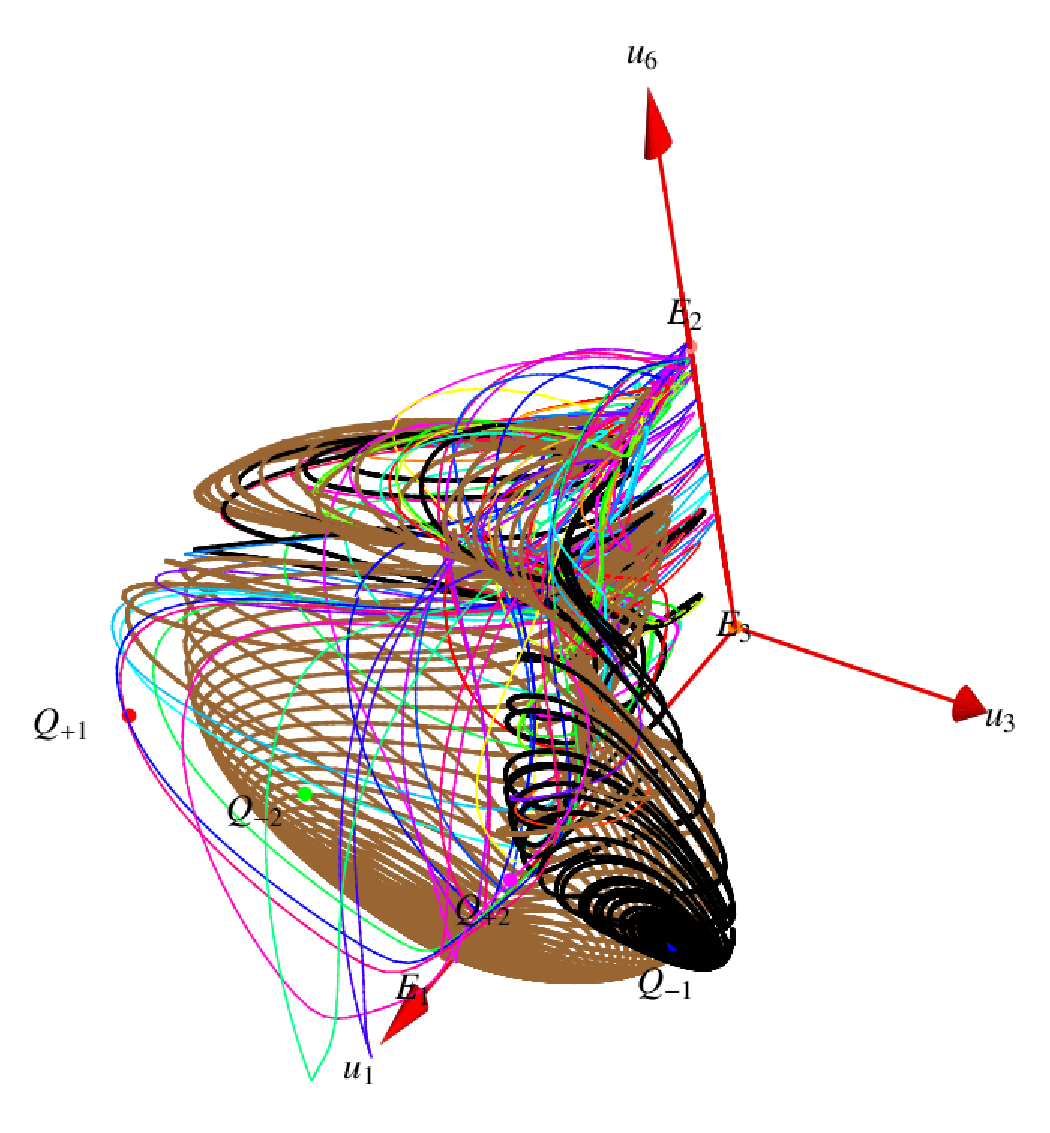
\includegraphics[width=0.35\textwidth]{../figs/ksSO2inv134.eps}
~~~~(\textit{b})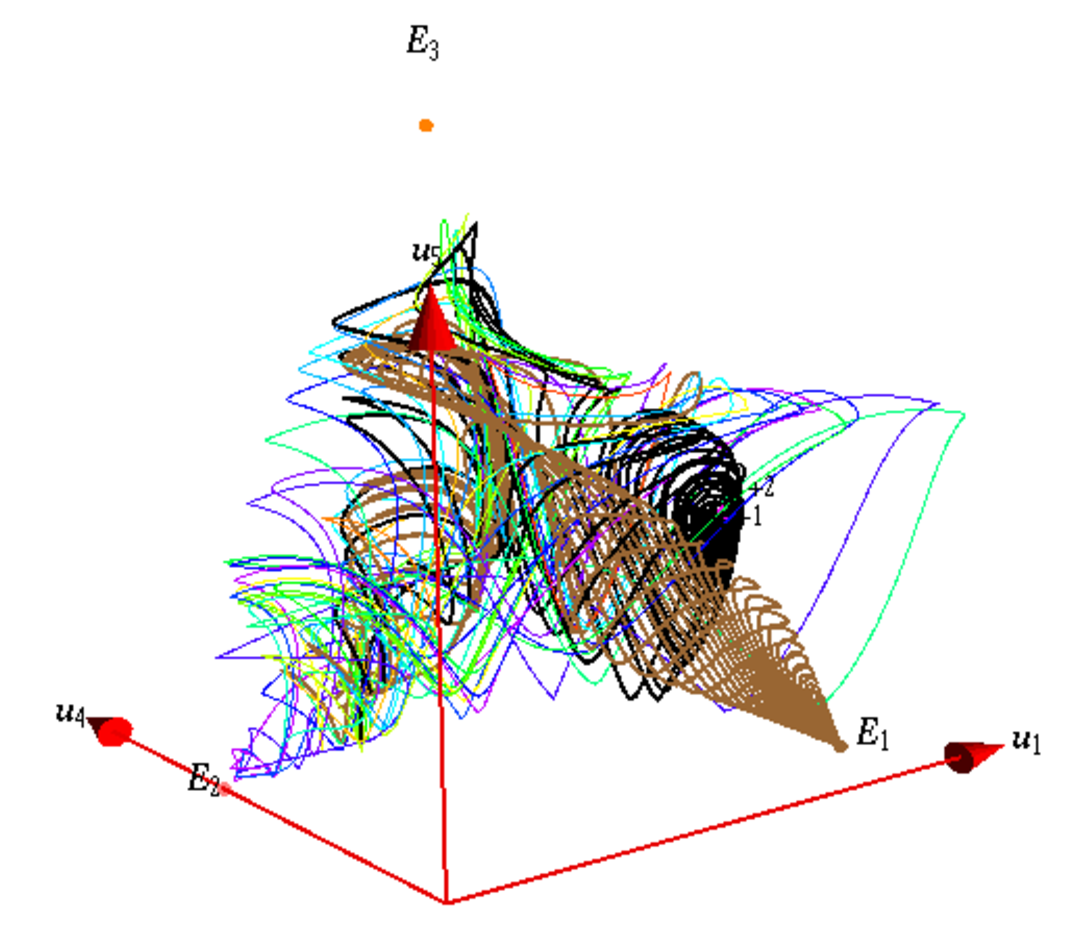
\includegraphics[width=0.35\textwidth]{../figs/ksSO2inv145.eps}
\end{center}
\caption[KSe SO(2) reduced phase space with second set of modified invariants.]{ Two different projections
of L=22 \KS\ dynamics on invariants given in \reftab{tab:SO2n6modif}. The trajectories shown are 20 short \rpo s. A trajectory on the unstable manifold of $\REQB{1}$ is shown in black.}
\label{fig:SO2inv}
\end{figure}
%%%%%%%%%%%%%%%%%%%%%%%%%%%%%%%%%%%%%%%%%%%%%%%%%%%%%%%%%%%%%%%%

 
